% Dokumentum konfiguráció
\documentclass[fleqn,12pt]{article}
% --------------------------------------------------
% Dokumentum adatok
% --------------------------------------------------

% Intézmény és kar
\newcommand\INTEZMENY{Budapesti Műszaki és Gazdaságtudományi Egyetem}
\newcommand\KAR{Gépészmérnöki Ka}
\newcommand\LOGO{bme-logo.jpg} % logo fájl neve a figures mappában

% Dokumentum adatok
\newcommand\CIM{Statik 3. Hausaufgabe}
\newcommand\DATUM{2025/26/1}
\newcommand\NEV{Abos Gergő}
\newcommand\NEPTUN{C46M9M}
\newcommand\EMAIL{gergo.abos@gmail.com}
\newcommand\TANTARGY{Statik}
\newcommand\TANTARGYKOD{BMEGEMMBXM1}

% --------------------------------------------------
% Preambulum és egyéni parancsok betöltése
% --------------------------------------------------

\input{../_settings/00_preambulum.tex}
\input{../_settings/01_commands.tex}
\usetikzlibrary{
  calc, % For coordinate calculations
  decorations.pathmorphing, % For support hatching
  patterns, % For filling (though not used here, opacity is)
  arrows.meta % For arrow tips
}

% ==================================================
% Dokumentum kezdete
% ==================================================
\begin{document}

% Címlap és tartalomjegyzék
% \input{contents/01_title.tex}
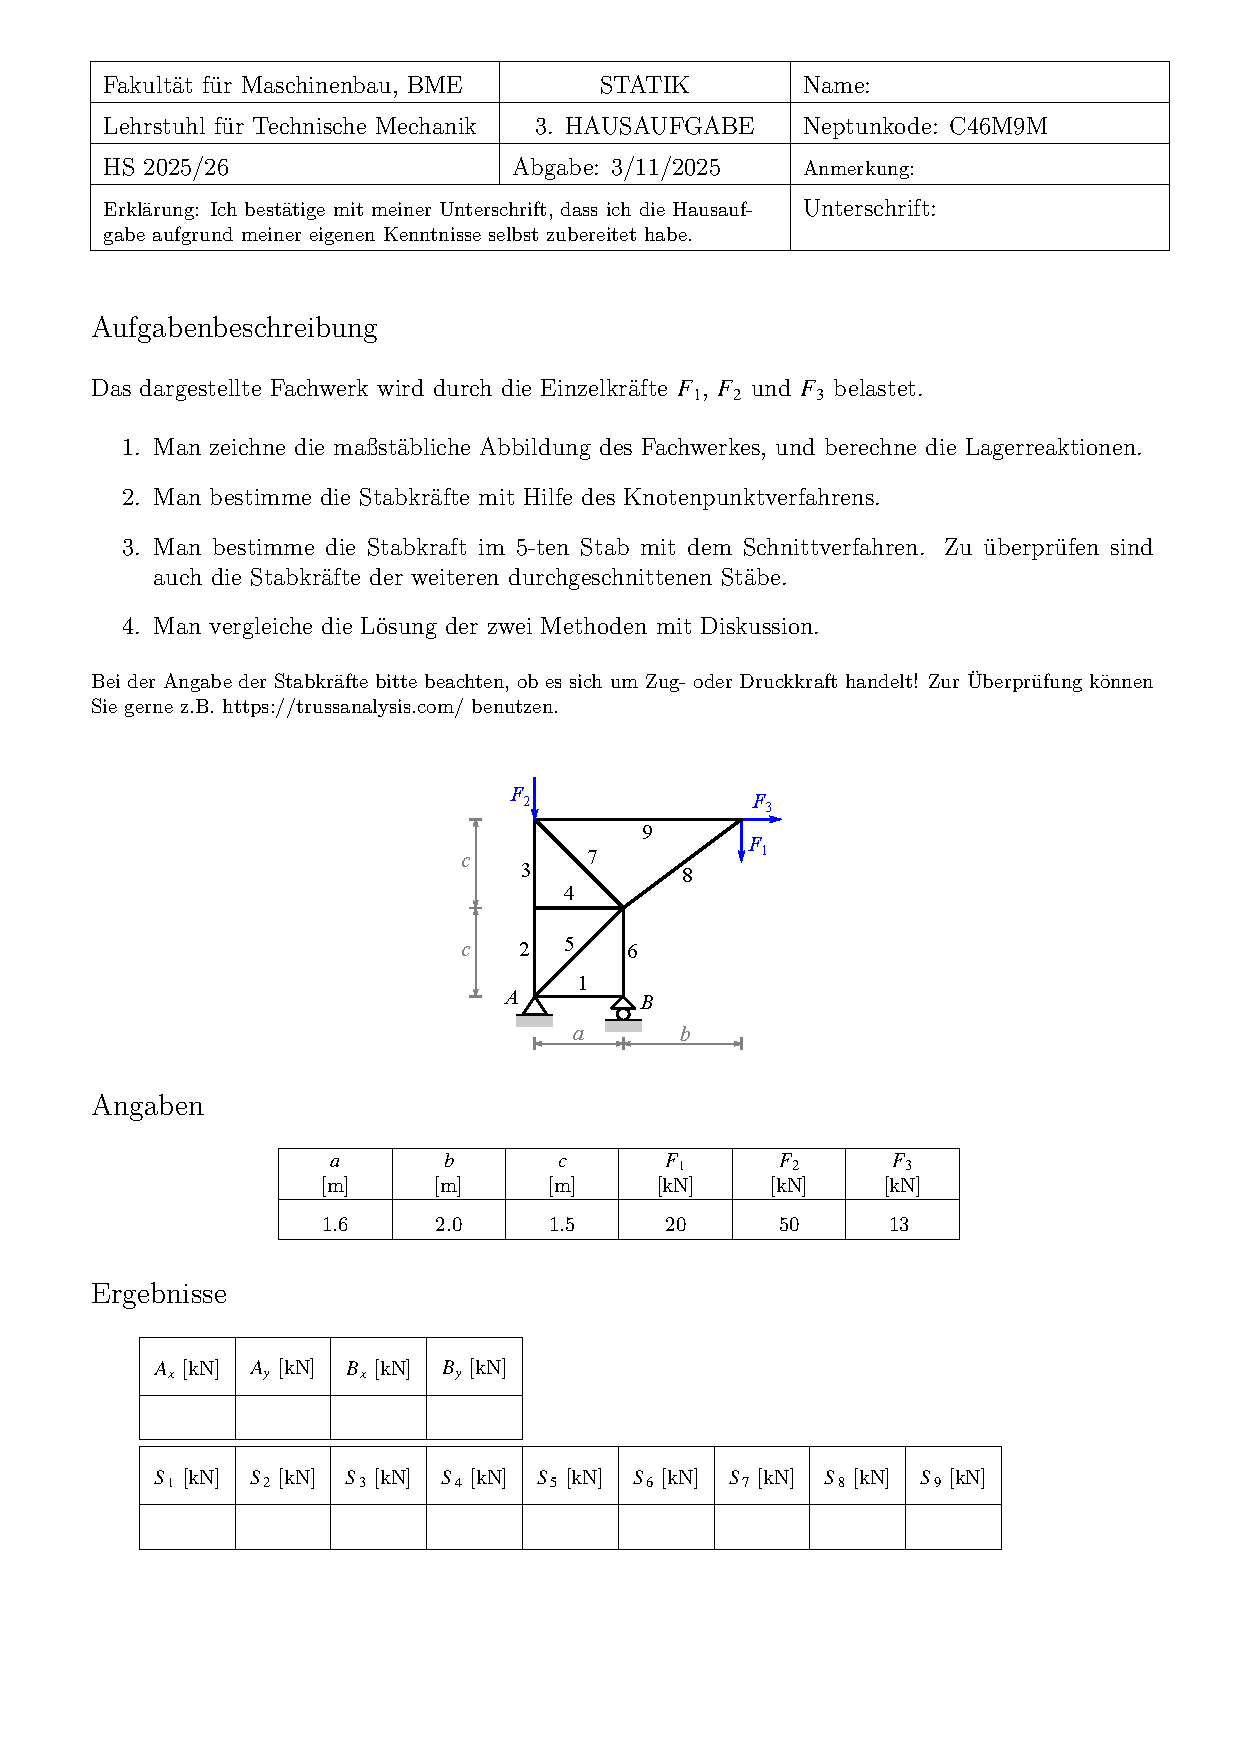
\includepdf[pages=1]{contents/stha3.pdf} % feladatlap beszúrása, ha szükséges
% \input{contents/02_contentpage.tex}
% --------------------------------------------------
% 0. fejezet
% --------------------------------------------------
\section{Maßstäbliche Abbildung, Lagerreaktionen}
\begin{figure}[h!]
  \centering
  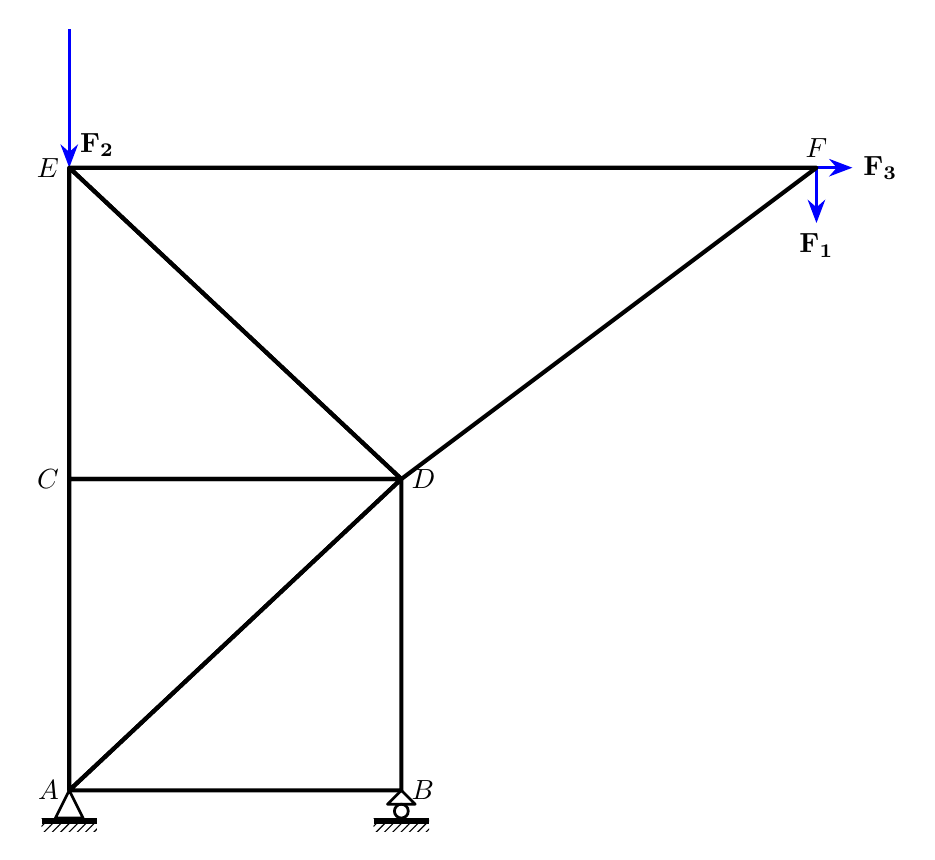
\begin{tikzpicture}[
      thick, % Default line thickness
      >=Stealth, % Default arrow tip
      force/.style={blue, very thick, ->}, % Style for force arrows
      dimline/.style={thin, <->, >=latex}, % Style for dimension lines
    ]

    % Größen
    \def\va{1.6pt * 75}
    \def\vb{2.0pt * 75}
    \def\vc{1.5pt * 75}
    \def\vfone{20pt}
    \def\vftwo{50pt}
    \def\vfthree{13pt}

    % Koordinaten von Punkte
    \coordinate (A) at (0, 0);
    \coordinate (B) at (\va, 0);
    \coordinate (C) at (0, \vc);
    \coordinate (D) at (\va, \vc);
    \coordinate (E) at (0, \vc * 2);
    \coordinate (F) at (\va + \vb, \vc * 2);

    % Beschriftungen von Punkte
    \node[left]  at (A) {$A$};
    \node[right] at (B) {$B$};
    \node[left]  at (C) {$C$};
    \node[right] at (D) {$D$};
    \node[left]  at (E) {$E$};
    \node[above] at (F) {$F$};

    % Lager in Punkt A
    \draw[draw=black, line width = 1pt, join=round] ($(A)$) -- ($(A) + (5pt, -10pt)$) -- ($(A) + (-5pt, -10pt)$) -- cycle;
    \draw[pattern=north east lines, pattern color=black, draw=none]
    ($ (A) + (-10pt, -10pt) $) rectangle ($ (A) + (10pt, -15pt) $);
    \draw[line width=2pt, black]
    ($ (A) + (-10pt, -11pt) $) -- ($ (A) + (10pt, -11pt) $);

    % Lager in Punkt B
    \draw[draw=black, line width = 1pt, join=round] ($(B)$) -- ($(B) + (5pt, -5pt)$) -- ($(B) + (-5pt, -5pt)$) -- cycle;
    \draw[draw=black, line width = 1pt] ($(B) + (0, -7.5pt)$) circle (2.5pt);
    \draw[pattern=north east lines, pattern color=black, draw=none]
    ($ (B) + (-10pt, -10pt) $) rectangle ($ (B) + (10pt, -15pt) $);
    \draw[line width=2pt, black]
    ($ (B) + (-10pt, -11pt) $) -- ($ (B) + (10pt, -11pt) $);

    % Kräfte
    \draw[force] (F) -- ($(F) + (\vfthree, 0)$)
    node[right, black] {$\mathbf{F_3}$};
    \draw[force] (F) -- ($(F) + (0, -\vfone)$)
    node[below, black] {$\mathbf{F_1}$};
    \draw[force] ($(E) + (0, \vftwo)$) -- (E)
    node[above right, black] {$\mathbf{F_2}$};

    % Fachwerk Stäber
    \foreach \i/\j/\k in {A/B/D, A/C/D, C/D/E, D/E/F}
    \draw[draw=black, line width = 1.5pt, join=round] (\i) -- (\j) -- (\k) -- cycle;

  \end{tikzpicture}
  \caption{Maßstäbliche Abbildung des Fachwerkes}
\end{figure}

Vor der Rechnungen zeichne ich erstmal ein Freiköperbild (\figref{fig:Freikörperbild}). Das Fachwerk wird als ein Starrkörper dargestellt, die Lager werden durch Reaktionskräfte ersetzt.

\begin{figure}[h!]
  \centering
  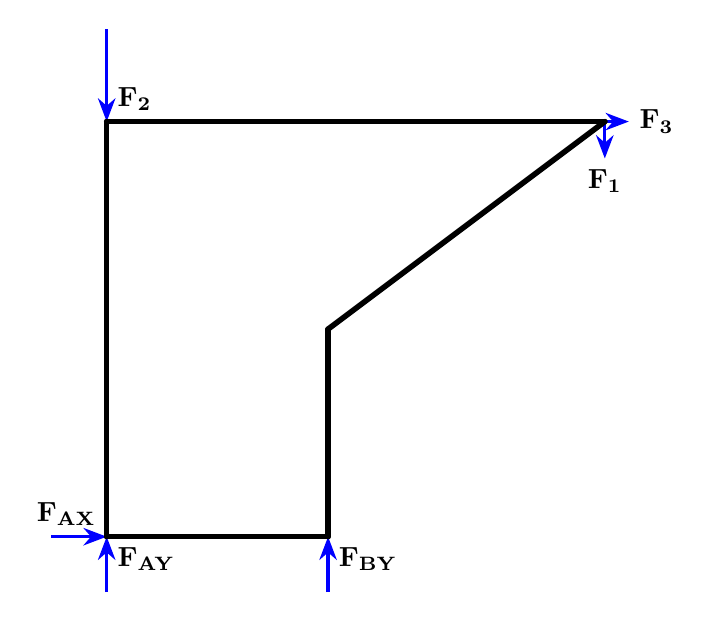
\begin{tikzpicture}[
      thick, % Default line thickness
      >=Stealth, % Default arrow tip
      force/.style={blue, very thick, ->}, % Style for force arrows
      dimline/.style={thin, <->, >=latex}, % Style for dimension lines
    ]

    % Größen
    \def\va{1.6pt * 50}
    \def\vb{2.0pt * 50}
    \def\vc{1.5pt * 50}
    \def\vfone{20pt * 2 / 3}
    \def\vftwo{50pt * 2 / 3}
    \def\vfthree{13pt * 2 / 3}

    % Koordinaten von Punkte
    \coordinate (A) at (0, 0);
    \coordinate (B) at (\va, 0);
    \coordinate (C) at (0, \vc);
    \coordinate (D) at (\va, \vc);
    \coordinate (E) at (0, \vc * 2);
    \coordinate (F) at (\va + \vb, \vc * 2);

    % Kräfte
    \draw[force] (F) -- ($(F) + (\vfthree, 0)$)
    node[right, black] {$\mathbf{F_3}$};
    \draw[force] (F) -- ($(F) + (0, -\vfone)$)
    node[below, black] {$\mathbf{F_1}$};
    \draw[force] ($(E) + (0, \vftwo)$) -- (E)
    node[above right, black] {$\mathbf{F_2}$};

    % Reaktionskräfte
    \draw[force] ($(A) + (0, -20pt)$) -- (A)
    node[above left, black] {$\mathbf{F_{AX}}$};
    \draw[force] ($(A) + (-20pt, 0)$) -- (A)
    node[below right, black] {$\mathbf{F_{AY}}$};
    \draw[force] ($(B) + (0, -20pt)$) -- (B)
    node[below right, black] {$\mathbf{F_{BY}}$};

    % Starrkörper
    \foreach \i/\j in {A/E, E/F, F/D, D/B, B/A}
    \draw[line width=2pt, black, cap=round] (\i) -- (\j);

  \end{tikzpicture}
  \caption{Freikörperbild}\label{fig:Freikörperbild}
\end{figure}
\pagebreak
Für einen im Gleichgewicht befindlichen Starrkörper gelten drei Gleichungen zur Bestimmung der Lagerreaktionen:
\begin{align}
  \label{eq:glgw1}
  &\sum F_X = F_{AX} + F_3 = 0 \\
  \label{eq:glgw2}
  &\sum F_Y = F_{AY} + F_{BY} - F_1 - F_2 = 0 \\
  \label{eq:glgw3}
  &\sum M_A = a \cdot F_{BY} - (a + b) \cdot F_1 - 2c \cdot F_3 = 0
\end{align}

Von \hyperref[eq:glgw1]{(\ref*{eq:glgw1})}:
\begin{align*}
  \boxed{F_{AX} = -13\,\text{kN}}
\end{align*}

Von \hyperref[eq:glgw2]{(\ref*{eq:glgw2})}:
\begin{align*}
  \boxed{F_{BY} = 69,375\,\text{kN}}
\end{align*}

Von \hyperref[eq:glgw3]{(\ref*{eq:glgw3})}:
\begin{align*}
  \boxed{F_{AY} = 0,625\,\text{kN}}
\end{align*}

\section{Stabkräfte mit Knotenpunktverfahren}

Da sich alle sechs (A-F) Knotenpunkte im Gleichgewicht befinden, gelten für jeden Punkt zwei Gleichungen:
\setcounter{equation}{0}
\begin{align}
  &\sum F_X = 0 \\
  &\sum F_Y = 0
\end{align}

1. Für Punkt B:
\begin{figure}[h!]
  \centering
  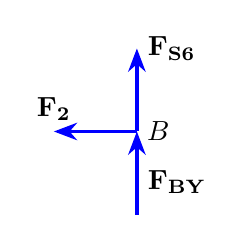
\begin{tikzpicture}[
      thick, % Default line thickness
      >=Stealth, % Default arrow tip
      force/.style={blue, very thick, ->}, % Style for force arrows
    ]
    % Größen
    \def\lange{30pt}
    % Koordinaten von Punkte
    \coordinate (O) at (0, 0);
    % Kräfte
    \draw[force] (O) -- ($(O) + (0, \lange)$)
    node[right, black] {$\mathbf{F_{S6}}$};
    \draw[force] ($(O) + (0, -\lange)$) -- (O)
    node[below right, black, yshift=-10pt] {$\mathbf{F_{BY}}$};
    \draw[force] (O) -- ($(O) + (-\lange, 0)$)
    node[above, black] {$\mathbf{F_2}$};
    %Punkt mit Beschrift
    \node[right]  at (O) {$B$};

  \end{tikzpicture}
\end{figure}
\begin{align*}
  &\sum F_X = F_{S1} = 0 & \sum F_Y = F_{BY} + F_{S6} = 0& \\
  &\boxed{F_{S1} = 0} & \boxed{F_{S6} = -69{,}375}&
\end{align*}

2. Für Punkt A:
\begin{figure}[h!]
  \centering
  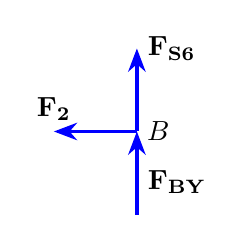
\begin{tikzpicture}[
      thick, % Default line thickness
      >=Stealth, % Default arrow tip
      force/.style={blue, very thick, ->}, % Style for force arrows
    ]
    % Größen
    \def\lange{30pt}
    % Koordinaten von Punkte
    \coordinate (O) at (0, 0);
    % Kräfte
    \draw[force] (O) -- ($(O) + (0, \lange)$)
    node[right, black] {$\mathbf{F_{S6}}$};
    \draw[force] ($(O) + (0, -\lange)$) -- (O)
    node[below right, black, yshift=-10pt] {$\mathbf{F_{BY}}$};
    \draw[force] (O) -- ($(O) + (-\lange, 0)$)
    node[above, black] {$\mathbf{F_2}$};
    %Punkt mit Beschrift
    \node[right]  at (O) {$B$};

  \end{tikzpicture}
\end{figure}
\begin{align*}
  &\sum F_X = F_{S1} = 0 & \sum F_Y = F_{BY} + F_{S6} = 0& \\
  &\boxed{F_{S1} = 0} & \boxed{F_{S6} = -69{,}375}&
\end{align*}
\end{document}
